\documentclass{article}
\usepackage[cm]{fullpage}
\usepackage[table]{xcolor}

\usepackage{csvsimple}

\usepackage{longtable}
\usepackage{booktabs}
\usepackage{tikz}
%\usepackage{colortbl}

\usepackage{calc}

\usepackage{multicol} 
\usepackage{float} %for the H placement
\usepackage{caption} %to hack captions into tikz without putting them inside figures that destroy multicol

\definecolor{earlgrey}{gray}{0.42}

\usepackage[unicode=true,pdfusetitle, bookmarks=true,bookmarksnumbered=false,bookmarksopen=false, breaklinks=false,pdfborder={0 0 0},backref=false,colorlinks=true,linkcolor = black,urlcolor = earlgrey] {hyperref}


%
%\documentclass[english]{article}
\usepackage[T1]{fontenc}
\usepackage[latin9]{inputenc}
%

%DRAFT WATERMARK (3lines)
%\usepackage{draftwatermark}
%\SetWatermarkText{\textbf{\textsf{Draft Report}}}
%\SetWatermarkScale{3.1416}


\usepackage{fancyhdr}
\usepackage{lastpage}

\pagestyle{fancy}
\fancyhf{}

\renewcommand{\headrulewidth}{0pt}
\renewcommand{\footrulewidth}{1pt}


\lfoot{PGP-UK Genomics Report for \input{SampleName.txt} [v19-257]}
\cfoot{\hspace{17em}\underline{Research use only}}
\rfoot{Page \thepage\ of \pageref{LastPage}}




\makeatletter



%%%%%%%%%%%%%%%%%%%%%%%%%%%%%% Hacky table solution.



% define lightgray
\definecolor{lightgray}{gray}{0.94}

% alternate rowcolors for all tables
\let\oldtabular\tabular
\let\endoldtabular\endtabular
\renewenvironment{tabular}{\rowcolors{2}{white}{lightgray}\oldtabular}{\endoldtabular}

% alternate rowcolors for all long-tables
\let\oldlongtable\longtable
\let\endoldlongtable\endlongtable
\renewenvironment{longtable}{\rowcolors{2}{white}{lightgray}\oldlongtable} {
\endoldlongtable}





%%%%%%%%%%%%%%%%%%%%%%%%%%%%%% User specified LaTeX commands.


\makeatother

\begin{document}

\title{PGP-UK Genomics Report for \input{SampleName.txt}}
\author{\vspace{-5ex}}
\date{\vspace{-5ex}}

\maketitle




%%%%%%%%%%%%%%%%%%% A few functions to start with

%\definecolorseries{myseries}{rgb}{step}[rgb]{.95,.85,.55}{.17,.47,.37} 
\definecolorseries{myseries}{hsb}{step}[hsb]{1,1,1}{.07,.89,.97} 
\resetcolorseries{myseries}%

% a pie slice
\newcommand{\slice}[4]{
     \pgfmathsetmacro{\midangle}{0.5*#1+0.5*#2}
     \begin{scope}
\clip (0,0) -- (#1:1) arc (#1:#2:1) -- cycle;
\colorlet{SliceColor}{myseries!!+}%
\fill[inner color=SliceColor!30,outer color=SliceColor!60] (0,0) circle (1cm);
     \end{scope}
     \draw[thick] (0,0) -- (#1:1) arc (#1:#2:1) -- cycle;
     \node[label=\midangle:#4] at (\midangle:1) {};
     \pgfmathsetmacro{\temp}{min((#2-#1-10)/110*(-0.3),0)}
     \pgfmathsetmacro{\innerpos}{max(\temp,-0.5) + 0.8}
     \node at (\midangle:\innerpos) {#3};
}


% make the full pie chart
\newcommand{\makechart}[2]{
    % sum of amounts
    \csvreader[before reading=\def\mysum{0}]{#1}{Count=\Count}{ %
    \pgfmathsetmacro{\mysum}{\mysum+\Count}%
    }
    %make picture itself

%\begin{figure}[H]
\begin{centering}

    \begin{tikzpicture}[scale=2.5]% 2.3 works well 
    \def\mya{0}\def\myb{0}
    \csvreader[head to column names]{#1}{}{\Label}
     }
    \end{tikzpicture}%
   \captionof{figure}{#2}

\par\end{centering}
%\caption{#2}
%\end{figure}

    
}


%%%%%%%%%%%%%%%%%%% Start of report

%\cofeAm{1}{1.0}{180}{5.5cm}{-7cm}


\section{Summary}

This is the genome report was produced using collaborative research tools, including \href{https://www.snpedia.com}{SNPedia} and \href{http://evidence.pgp-hms.org/about}{GetEvidence}. This section shows an overview of all the small variants which were found in the genome for this individual, when compared with a \href{http://www.ncbi.nlm.nih.gov/projects/genome/assembly/grc/human/}{reference genome}. These variants are summarised in Table 1 and the pie-charts in Figures 2, 3 and 4.
\par
This report was generated automatically and is not clinically approved. It is provided for \underline{personal and research purposes} \underline{only}. 
%If you have any concerns regarding the information present here, please consult a genetic counsellor or your general practitioner.
\par
This document contains hyperlinks, shown in \textcolor{earlgrey}{grey}, that will take you to external websites where you can find more detailed explanations. Some of the technical terms are also explained in more detail in the \href{http://www.ensembl.org/Help/Glossary}{Ensembl Glossary}. We would welcome your feedback about this report, for example, if you would like more information about anything or if any of the links have become inactive. You can contact us on: \href{mailto:pgp-uk@ucl.ac.uk}{pgp-uk@ucl.ac.uk}.
\par
\par
This summary shows an overview of all the variants which were found in the genome for this individual. The "variants remaining after filtering" refers to any differences in the DNA identified when compared to the reference genome. Of these, the majority will have already been found in some other sequenced individual and put on a database (existing variants) while others have not yet been annotated (novel variants). 
\par
 "Overlapped genes" refers to the number of times where a variant was found in a region of the genome containing a gene. The diagram in Figure 1 is a simplification of the usual gene structure.
 "Exon" refers to the part of the gene which goes on to form a protein, and variants in this part of the gene are more likely to cause changes in the shape of the protein. Upstream, downstream, intronic and intergenic variants are more likely to alter the regulation of that gene but will not change the protein itself.
\par
A transcript for a protein-coding gene can include the exons, introns and other gene features that are transcribed and important for gene function but might not be translated into the final protein. Not all transcripts are for protein-coding genes, with many containing non-coding RNAs that can be overlapping other genes, in introns or in intergenic regions.
\vspace{5 mm}

\begin{figure}[H]
\begin{centering}
%\includegraphics[width=0.95\textwidth]{geneplot.jpeg}
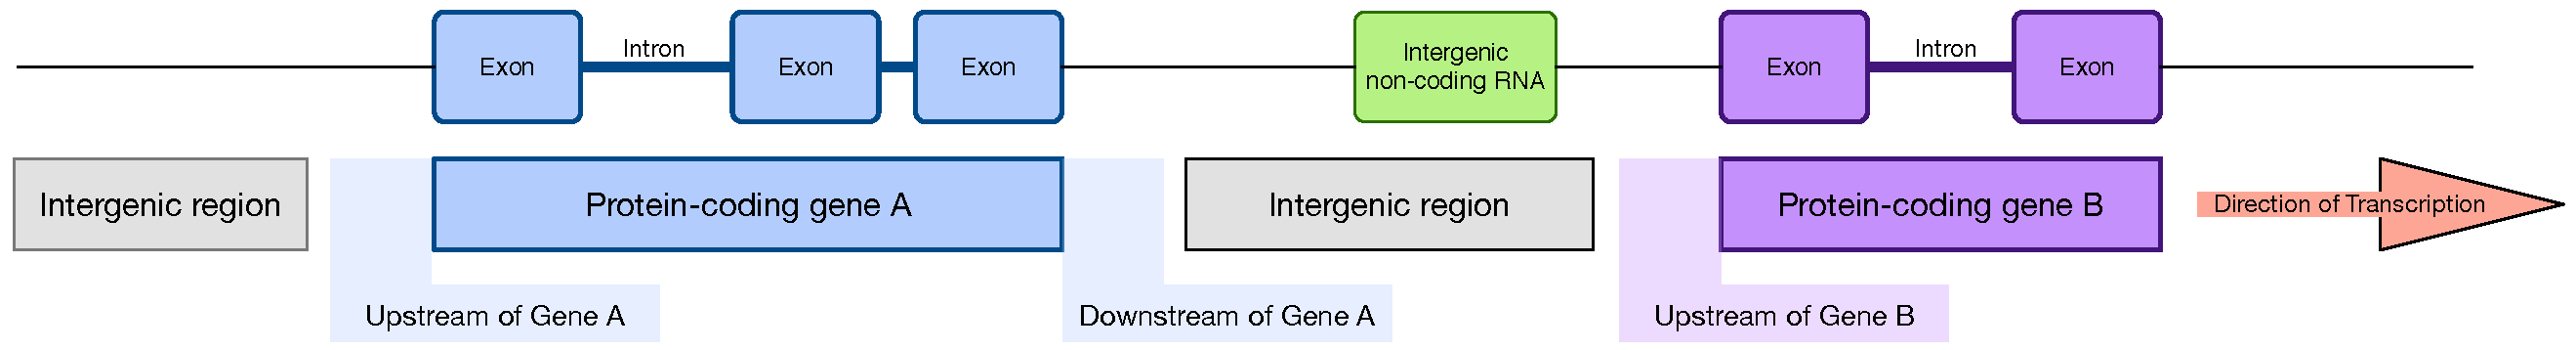
\includegraphics[width=0.99\textwidth]{GeneStructure.pdf}
\par\end{centering}

\caption{Diagram of gene structure indicating locations of potential variants}
\end{figure}


\pagebreak

\section{Ancestry}

This plot shows the distribution of the genomes of different populations. Data from several studies which used whole genome sequencing was used to see the relationships between the genomes of the populations. It shows how closely related certain populations are genetically: Groups which cluster closely are more genetically similar than groups which are further apart. The black star symbol shows where this PGP-UK participant sits in relation to other populations, indicating their ancestry and their most closely related populations according to genetic sequence.
\par
Please note that this analysis is limited by the populations available in the  \href{http://www.internationalgenome.org/category/population/}{1000 genomes project} (1kGP) data. If there are European subpopulations reported, and the ancestry of the participant does not correspond to any of the 1kGP populations, the closest 1kGP sampled subpopulation will be shown (even though it might be different from the participant's actual ancestry).


\vspace{15 mm}


\begin{figure}[H]
\begin{centering}
\includegraphics[width=0.85\textwidth]{AncestryPlot.pdf}
\par\end{centering}

\caption{Ancestry Principal Component Analysis}
\end{figure}



\pagebreak



\section{Traits (based on SNPedia information)}

Existing research has associated many variants with phenotypic traits, some of which can be perceived as beneficial while others appear to have a harmful effect. Some traits are complex and can be affected by several variants. It is likely that some of these would confer a higher risk while others a lower risk of trait manifestation. These can not be combined linearly to produce an actual risk of disease. 
\par
It is important to note that in most cases genomic data is probabilistic, not deterministic- i.e. having a genetic predisposition for a disease is not a diagnosis; rather, it shows an increased likelihood of developing that disease. Also, one person can have both potentially beneficial and harmful variants in the same gene, or associated with the same disease. 
\par
Some variants can also affect certain populations more, or will only affect a particular gender. For example, a variant for higher risk of endometriosis in the sequence of a male will not directly affect that person, but can be passed on to descendants.  
\par
While many traits are the result of a unique variant, many are the combination of several variants throughout the genome. In SNPedia, these are called  \href{https://www.snpedia.com/index.php/Genoset}{genosets}. These can integrate some of the information already present in the single variant tables, or be the combination of variants that have no phenotypic effect on their own, but contribute to a trait when together.
\par
The variants in the following tables are sorted by magnitude. This is an subjective measure defined in \href{https://www.snpedia.com}{SNPedia} to highlight the perceived importance of the genotype described. At the moment this scale goes from 0 to 10. You can read more about it by visiting their explanatory \href{https://www.snpedia.com/index.php/Magnitude}{webpage}.
\par
As our knowledge grows, the interpretation of the effect of certain variants might change. Clicking on the links in the genome report tables will take you to websites containing more information about each variant.

\vspace{15 mm}

%\begin{itemize}
%\item {\large Possibly Beneficial Traits}
%\end{itemize}
\subsection{Possibly Beneficial Traits}

\csvautolongtable[respect all,respect backslash=false,respect leftbrace=false,respect rightbrace=false,separator=comma]{latest.good.reportTable.csv}


\pagebreak


\subsection{Possibly Harmful Traits}

\csvautolongtable[respect all,respect backslash=false,respect leftbrace=false,respect rightbrace=false,separator=comma]{latest.bad.reportTable.csv}


\pagebreak

\subsection{Genosets (Multi-variant Phenotypes)}


\csvautolongtable[respect all,respect backslash=false,respect leftbrace=false,respect rightbrace=false,separator=comma]{latest.genoset.reportTable.csv}


\section{Report Metadata}

\begin{table}[H] %H
\begin{centering}
%\csvautotabular[ respect all,respect backslash=false,respect leftbrace=false,respect rightbrace=false,separator=comma]{versionTable.txt}
\csvautotabular[respect all,respect backslash=false,respect leftbrace=false,respect rightbrace=false,separator=tab]{versionTable.txt}
\par\end{centering}
\caption{Analysis Pipeline Versions}
\end{table}

\par
Report generated on \today. %v1 was 16-116

\end{document}
